
\pgfplotsset{every axis/.append style={
                    %axis x line=middle,    % put the x axis in the middle
                    %axis y line=middle,    % put the y axis in the middle
                    axis line style={-,color=LightBlue}, % arrows on the axis
                    xlabel={time},          % default put x on x-axis
                    ylabel={scale of the universe},          % default put y on y-axis
            }}



\begin{frameb}{w}{Images/HubbleXDF.png}
	\frametitle{Dark Energy}
	\framesubtitle{The Problem}
\end{frameb}


\begin{frame}
	\frametitle{The evolution of the universe}
	\framesubtitle{Three options:}
\begin{tikzpicture}
    \begin{axis}[
	    ticks=none,
	    width=\textwidth,
	    height=0.8\textheight,
            xmin=0,xmax=6.282,
            ymin=0,ymax=4,
            ]
            \addplot [domain=0:6.282,samples=50]({x-sin(180*x/3.141)},{1-cos(180*x/3.141)}); 
            \addplot [domain=0:7,samples=50]({(x^3)/6.},{(x^2)/2.}); 
            \addplot [domain=0:3,samples=50]({sinh(x)-x},{cosh(x)-1}); 
    \end{axis}
    \draw(0.95\textwidth,0) node [below left] {big crunch};
    \draw(0,0) node [below right] {big bang};
    \draw(0.375\textwidth,0.625\textheight) node [above left] {expands forever};
    \draw(0.475\textwidth,0.625\textheight) node [above right] {\em only just};
\end{tikzpicture}
\end{frame}




\begin{frameb}{w}{Images/tycho.jpg}
	\frametitle{Dark Energy}
	\framesubtitle{The Problem}
\end{frameb}


\begin{frame}
	\frametitle{The evolution of the universe}
	\framesubtitle{Three options:}
\begin{tikzpicture}
    \begin{axis}[
	    ticks=none,
	    width=0.9\textwidth,
	    height=0.8\textheight,
            xmin=0,xmax=6.282,
            ymin=0,ymax=20,
            ]
            \addplot [domain=0:6.282,samples=50]({x-sin(180*x/3.141)},{1-cos(180*x/3.141)}); 
            \addplot [domain=0:7,samples=50]({(x^3)/6.},{(x^2)/2.}); 
            \addplot [domain=0:3,samples=50]({sinh(x)-x},{cosh(x)-1}); 
    \end{axis}
    \draw(0.95\textwidth,0) node [below left] {big crunch};
    \draw(0,0) node [below right] {big bang};
    \draw(0.95\textwidth,0.3\textheight) node [left] {expands forever};
    \draw(0.9\textwidth,0.17\textheight) node [left] {\em only just};
\end{tikzpicture}
\end{frame}


\begin{frame}
	\frametitle{The evolution of the universe}
	\framesubtitle{None of the above:}
\begin{tikzpicture}
    \begin{axis}[
	    ticks=none,
	    width=0.9\textwidth,
	    height=0.8\textheight,
            xmin=0,xmax=6.282,
            ymin=0,ymax=20,
            ]
            \addplot [domain=0:6.282,samples=50]({x-sin(180*x/3.141)},{1-cos(180*x/3.141)}); 
            \addplot [domain=0:7,samples=50]({(x^3)/6.},{(x^2)/2.}); 
            \addplot [domain=0:3,samples=50]({sinh(x)-x},{cosh(x)-1}); 
	    \addplot [domain=0:5,samples=50]({x},{(3)^(1/3)*sinh(x)^(2/3)}); 
    \end{axis}
    \draw(0.95\textwidth,0) node [below left] {big crunch};
    \draw(0,0) node [below right] {big bang};
    \draw(0.95\textwidth,0.3\textheight) node [left] {expands forever};
    \draw(0.9\textwidth,0.17\textheight) node [left] {\em only just};
    \draw(0.475\textwidth,0.625\textheight) node [above right] {accelerated expansion};
\end{tikzpicture}
\end{frame}

\begin{frame}
	\frametitle{Dark Energy}
	\framesubtitle{The Problem}
	\begin{itemize}
		\item The Universe isn't slowing down in its expansion, but {\em speeding up!}
		\pause\item One of the ways in which this could happen would be the presence of an energy permeating the universe, accelerating the expansion.
		\pause\item We call this Dark Energy
		\pause\item Like Dark Matter, it's really just a name for a phenomenon which we observe, and haven't been able to explain yet
	\end{itemize}
\end{frame}

\begin{frame}
	\frametitle{Dark Energy\ldots}
	\framesubtitle{\ldots or Cosmological Constant?}

	\begin{columns}
	\begin{column}{0.5\textwidth}
		\begin{itemize}
			\item<1-> Einstein's gravity can be repulsive at large scales.
			\item<2-> This is known as a cosmological constant.
			\item<3-> In modern terms, we think of it as a type of energy.
		\end{itemize}
	\end{column}
	\begin{column}{0.5\textwidth}
	\begin{tikzpicture}
	  	\node (img1) {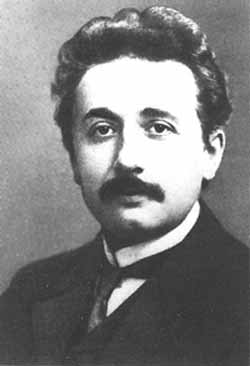
\includegraphics[height=4cm]{Images/young_einstein.jpg}};
	  	\pause
		\node (img2) at (img1.south east) [xshift=1cm] {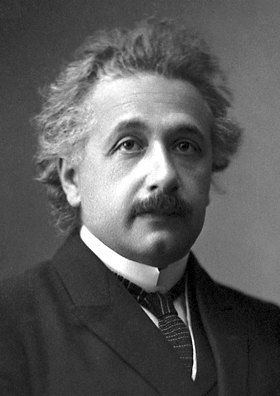
\includegraphics[height=4cm]{Images/nobel_einstein.png}};
	  	\pause
	  	\node (img3) at (img2.south west) [xshift=-1cm,yshift=1cm] {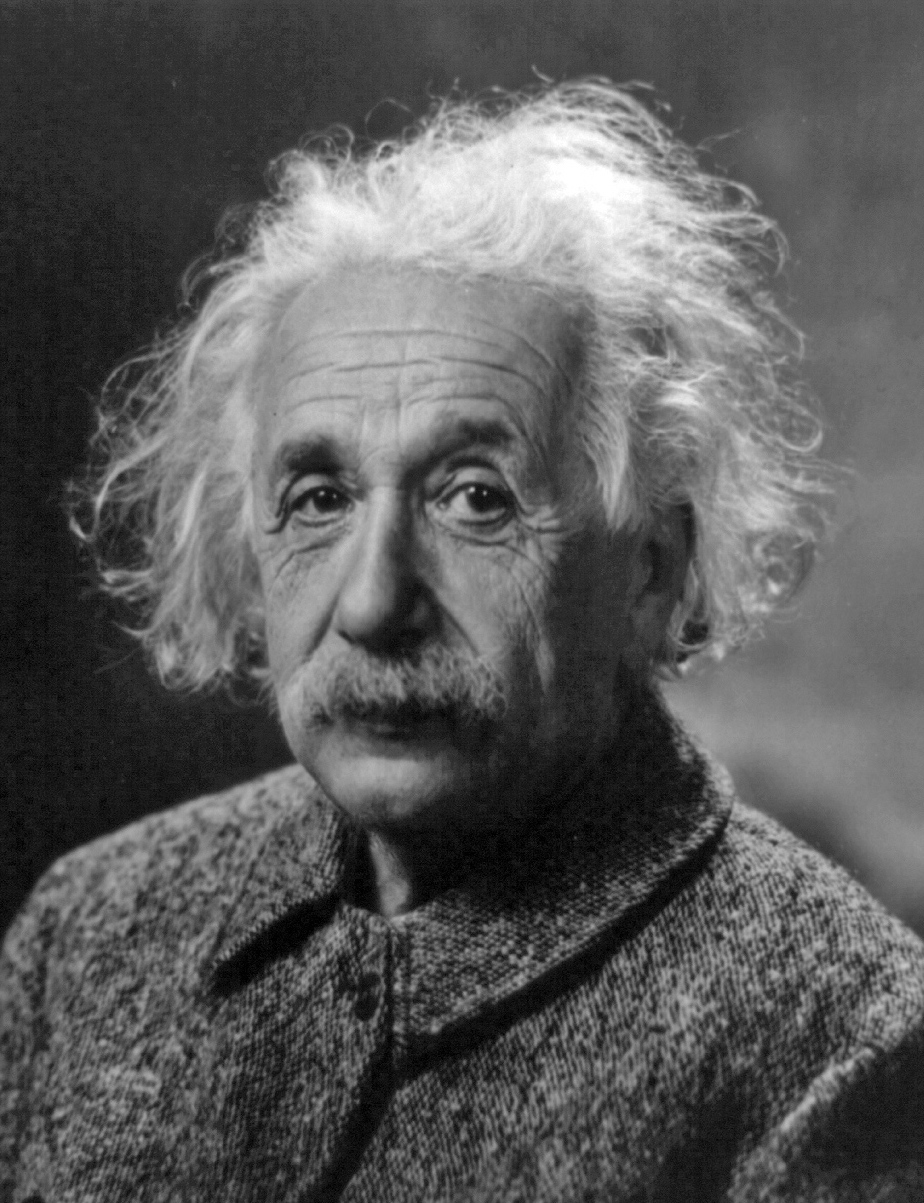
\includegraphics[height=4cm]{Images/old_einstein.jpg}};
	\end{tikzpicture}
	\end{column}
	\end{columns}
	
\end{frame}


\begin{frameb}{h}{Images/Euclid_telescope.jpg}
	\frametitle{The Euclid Satellite}
	\framesubtitle{Exploring dark energy}

\begin{columns}
\begin{column}{0.6\textwidth}
	\vspace{60pt}
	\begin{itemize}
		\pause\item Launch date $\approx 2020$
		\pause\item Build up an accurate 4D picture of the visible universe
		\pause\item By measuring cosmic shear around galaxies and clusters, will be able to build up a map of Dark Matter
		\pause\item Will see any variation in dark energy across space and time, enabling us to build a better understanding of it. 
	\end{itemize}
\end{column}
\begin{column}{0.4\textwidth}
\end{column}
\end{columns}
	
\end{frameb}




